\documentclass{article}[jsarticle]
\usepackage[T1]{fontenc}
\usepackage[dvipdfmx]{hyperref}
\usepackage{lmodern}
\usepackage{latexsym}
\usepackage{amsfonts}
\usepackage{amssymb}
\usepackage{mathtools}
\usepackage{nccmath}
\usepackage{amsthm}
\usepackage{multirow}
\usepackage[dvipdfmx]{graphicx}
\usepackage{wrapfig}
\usepackage{here}
\usepackage{float}
\usepackage{ascmac}
\usepackage{url}

\title{機械学習 課題1}
\author{高林秀 \\ 三宅研究室 博士前期課程1年 \\ V-CampusID : 23vr008n}
\date{\today}

\begin{document}

\maketitle

\begin{abstract}
    \noindent
    本稿は本年度必修授業の機械学習の第1回レポートの答案用紙である。\par
    \noindent
    本稿は、第1回授業~第4回授業までの範囲を対象とし、各回で課された課題に対する解答を記載する。\par
    \noindent
    答案の問題番号は各章のタイトルに記載している。\par
    \noindent
    各問に対する解答は本稿に、コードなどの実行結果は別途GoogleColaboratoryのノートブックに記載した
    巻末の付録から参照できる。
\end{abstract}

\section{第1回授業 : 4/11 宿題1}
    \subsection{問題文}
    二つのデータ点の近さを測る定量的指標の一つとして距離がある。いま、次の三つのデータ点があるとする
    \begin{flalign}
        & \text{データ点1} : (5,2,5.8) \\
        & \text{データ点2} : (7, 10, 1, 12) \\
        & \text{データ点3} : (3, 2, 6, 3)
    \end{flalign}
    上の各データ点は4種類の計測値で与えられている(例えば「緯度、経度、水深、温度」のような感じ)。
    このデータ点同士の間の近さをユークリッド距離で計算し、互いの距離が近いペアの順番を答えよ。データが近いほど距離が小さいことに注意。
    
    \subsection{解答}
    データ点の近さは以下の順番である。
    \begin{enumerate}
        \item データ店1とデータ点3、距離 : $5.4$
        \item データ店1とデータ点2、距離 : $10.0$
        \item データ店2とデータ点3、距離 : $13.6$
    \end{enumerate}
    ユークリッド距離は以下の式で計算できる。
    \begin{flalign*}
        & d(x,y) :\text{データ点xとデータ点yの距離として、}\\
        & d(x,y) = \sqrt{\sum_{i=1}^{n}(x_i - y_i)^2} \\
        & \text{※}x_i,y_i\text{はそれぞれデータ点}x,y\text{のi番目の要素を表す}
    \end{flalign*}
    各点間の距離は以下のように計算できる %TODO:後で手計算すること
    \begin{flalign*}
        & d(1,3) = \sqrt{(5-3)^2 + (2-2)^2 + (5.8-6)^2 + (0-3)^2} = 5.4 \\
        & d(1,2) = \sqrt{(5-7)^2 + (2-10)^2 + (5.8-1)^2 + (0-12)^2} = 10.0 \\
        & d(2,3) = \sqrt{(7-3)^2 + (10-2)^2 + (1-6)^2 + (12-3)^2} = 13.6
    \end{flalign*}

\section{第2回授業 : 4/18 宿題2}
    \subsection{問題文}
    \begin{figure}[H]
        \centering
        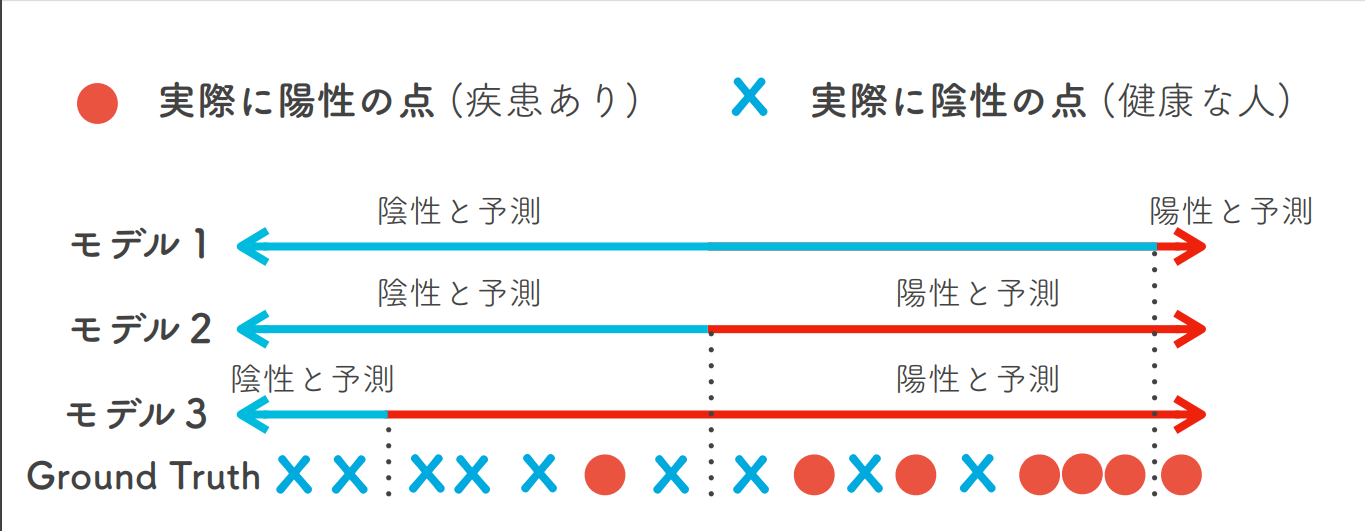
\includegraphics[scale=0.7]{./images/MLQ2.png}
    \end{figure}
    \begin{enumerate}
        \item 上の三つの分類モデルそれぞれに対し、混同行列、Precision、Recallを計算しなさい。
        \item モデル1→モデル2→モデル3の順に、Precisionは増加や減少の傾向にあるでしょうか?その傾向はなぜ生じるでしょう?また、Recallについても傾向はどうなっていますか?Precisionの傾向と対比して議論して見てください。
    \end{enumerate}
    
    \subsection{解答}

\section{第3回授業 : }
\section{第4回授業 : }

\section{付録}
\begin{itemize}
    \item GoogleColabノートブック : 
    \item 提出用GoogleDriveフォルダ : 
\end{itemize}
\end{document}